\documentclass{beamer}

\usetheme{Boadilla}
\usecolortheme{beaver}

\usepackage{mathtools}
\usepackage{derivative}
\usepackage{tikz-cd}

\usepackage{graphicx}
\graphicspath{ {./images/} }

\DeclareMathOperator{\coker}{coker}
\DeclareMathOperator{\Hom}{Hom}
\DeclareMathOperator{\Tot}{Tot}
\DeclareMathOperator{\Coh}{Coh}
\DeclareMathOperator{\Crit}{Crit}
\DeclareMathOperator{\MF}{MF}

\newcommand{\A}{\mathbb{A}}
\newcommand{\C}{\mathbb{C}}
\newcommand{\Z}{\mathbb{Z}}
\renewcommand{\P}{\mathbb{P}}
\renewcommand{\O}{\mathcal{O}}
\newcommand{\calA}{\mathcal{A}}
\newcommand{\calB}{\mathcal{B}}
\newcommand{\calC}{\mathcal{C}}
\newcommand{\calD}{\mathcal{D}}
\newcommand{\calP}{\mathcal{P}}
\newcommand{\calE}{\mathcal{E}}
\newcommand{\calF}{\mathcal{F}}

\newcommand{\dL}[1]{\mathbf{L}#1}
\newcommand{\dR}[1]{\mathbf{R}#1}
\DeclareMathOperator{\RHom}{\dR Hom}

\newcommand{\id}{\mathrm{id}}
\newcommand{\pt}{\mathrm{pt}}

\title{Derived categories of coherent sheaves}
\subtitle{(and matrix factorizations)}
\date{15th May 2024}
\author{Calum Crossley}

\begin{document}

\begin{frame}
    \titlepage
\end{frame}

\begin{frame}
    \frametitle{Overview}

    \begin{itemize}
        \item Introduce derived categories of coherent sheaves

            (setting: smooth projective varieties over $\C$) \pause

        \item Look at matrix factorizations

            (setting: affine hypersurface singularities) \pause

        \item Two theorems: Kn\"orrer periodicity, cone singularities

            (relate matrix factorizations and derived categories)
    \end{itemize}
\end{frame}

\section{Derived categories of coherent sheaves}

\begin{frame}
    \frametitle{Coherent sheaves}

    Smooth projective variety $X/\C$. \pause

    ~

    Vector bundles (locally free sheaves): $\O^{\oplus 3}$, $\O(-1)$, $\ldots$
    \pause

    ~

    Coherent sheaves = (finite rank) vector bundles + cokernels

    $\to$ abelian category \pause

    ~

    Think vector bundles on subvarieties (sheaf pushforward), e.g. $\O_\pt$

    \begin{center}
        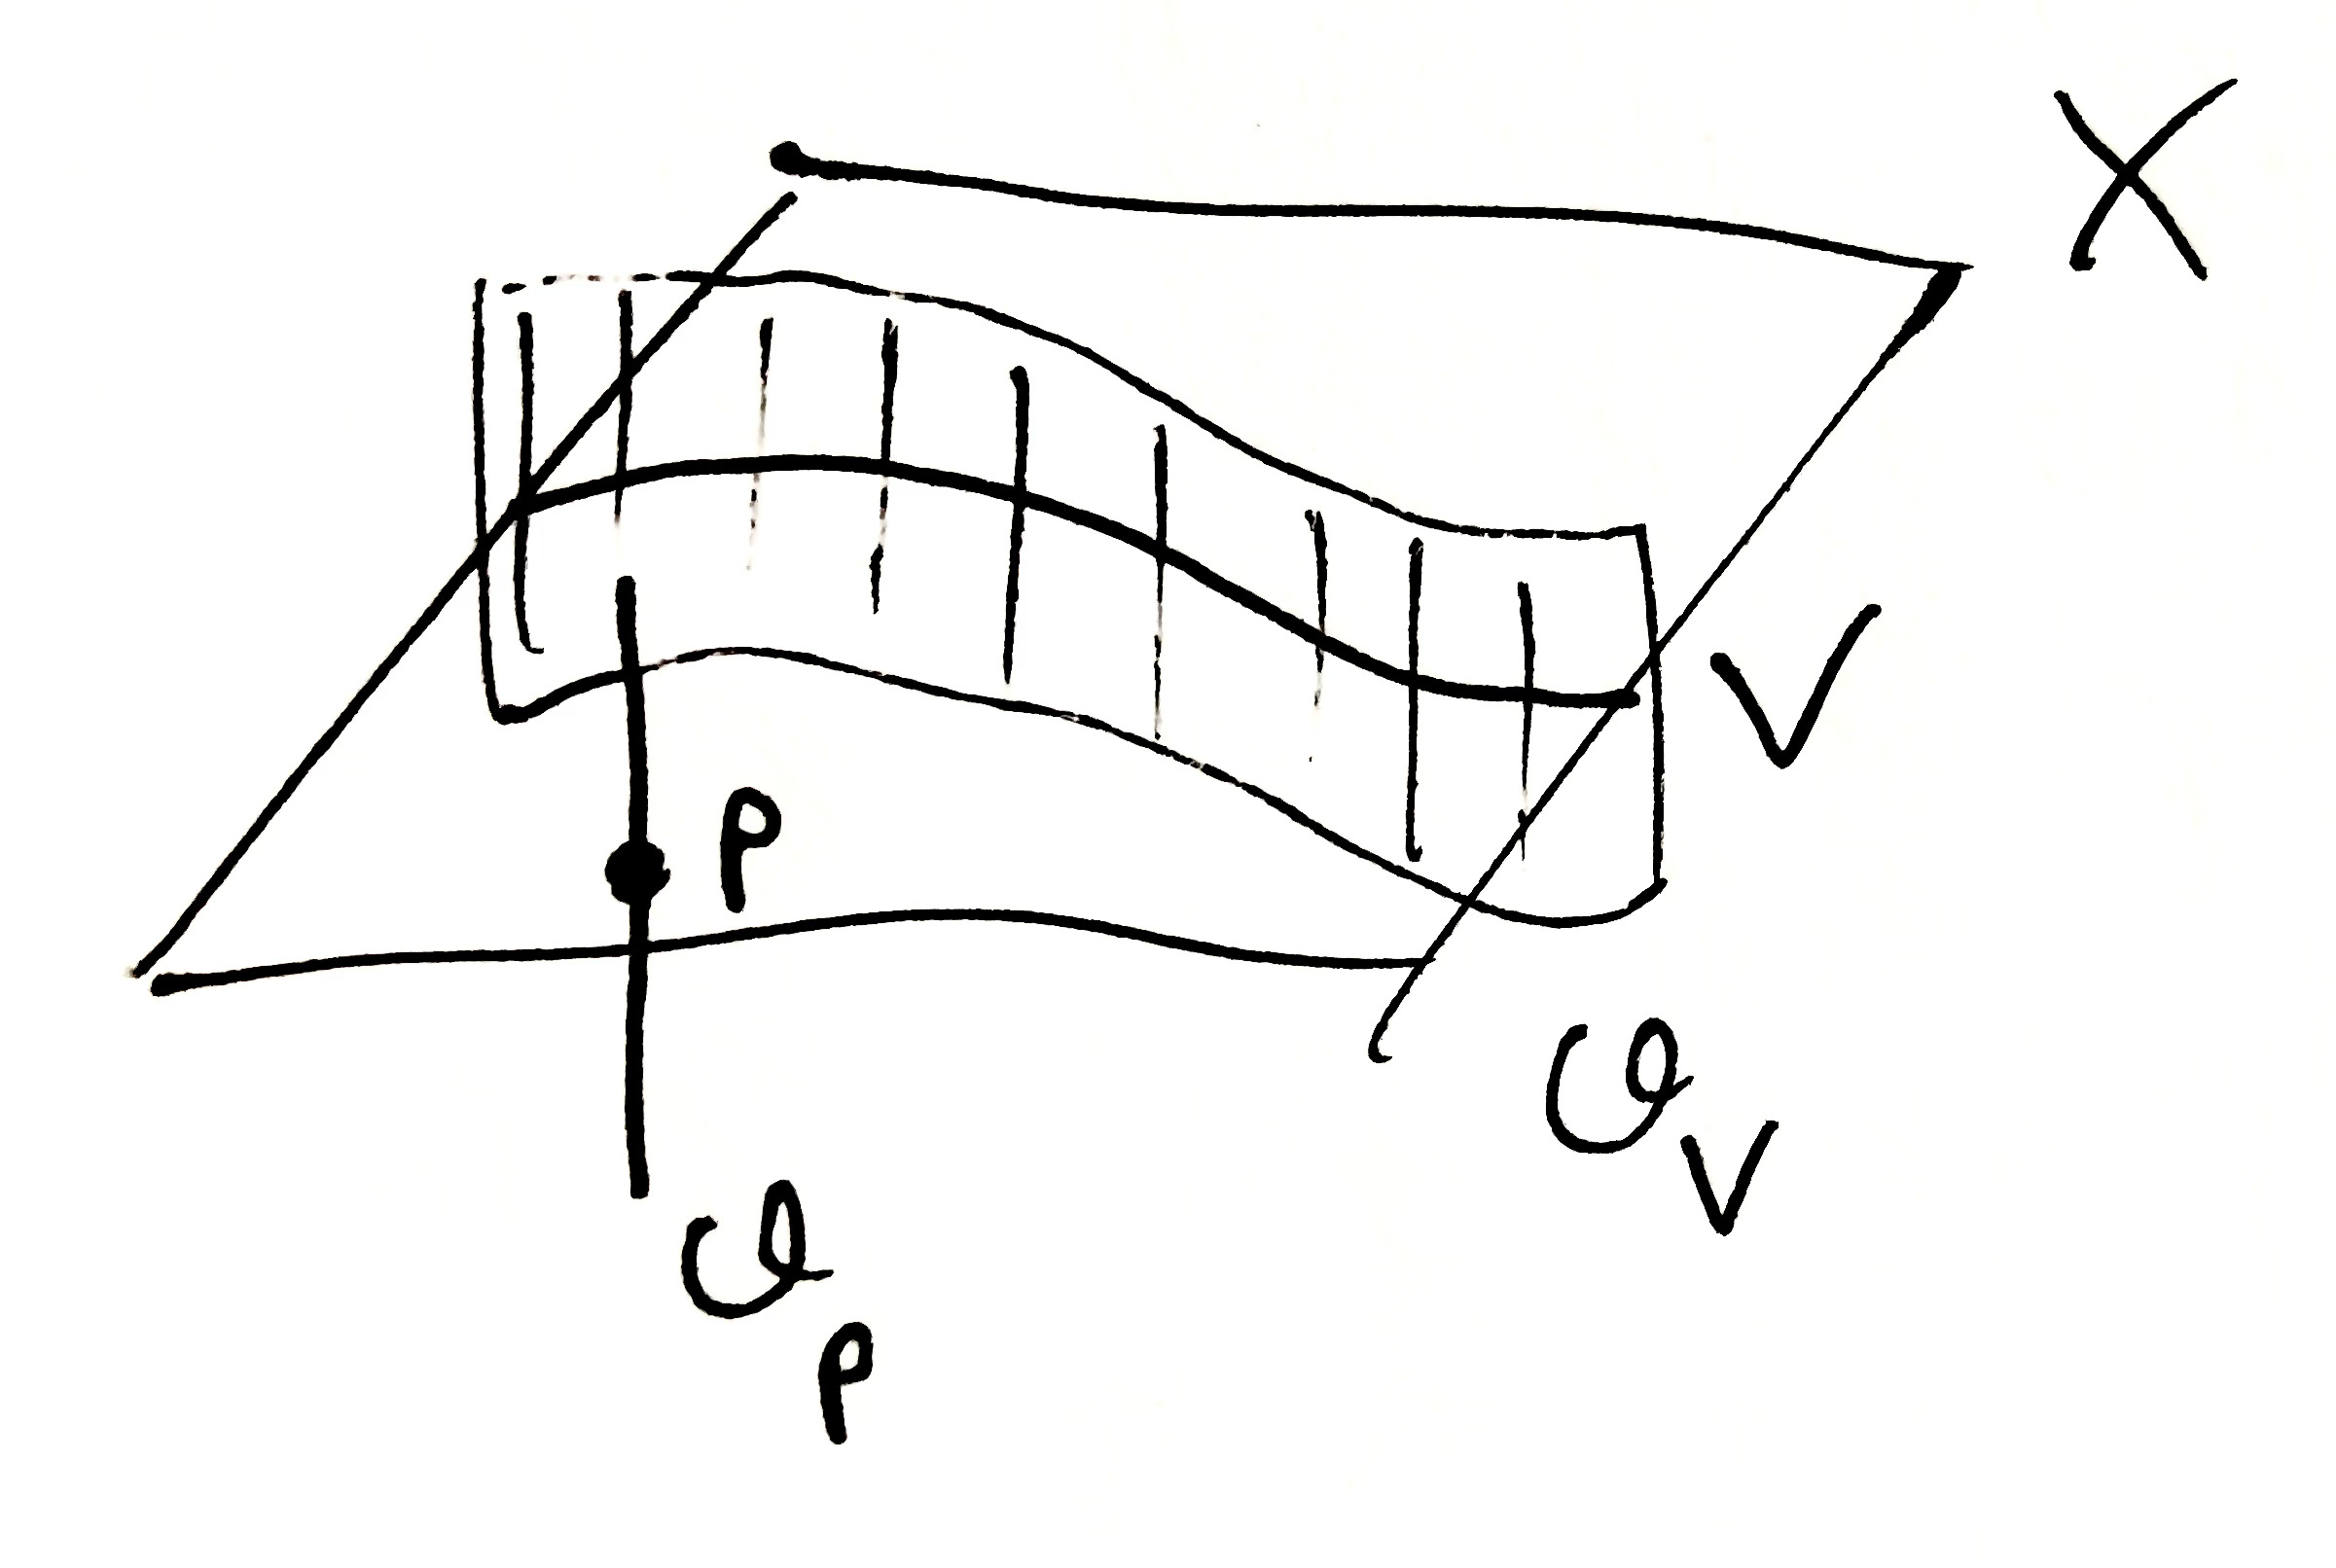
\includegraphics[scale=0.05]{coherent_sheaves}
    \end{center} \pause

    $\to$ $\Coh(X)$, determines $X$ (Gabriel-Rosenberg reconstruction)
    % technically that's QCoh, but Coh result also holds after Gabriel's results
    % Buan-Krause-Solberg, Support varieties -- an ideal approach, section 8
    % Garkusha-Prest, reconstructing projective schemes
\end{frame}

\begin{frame}
    \frametitle{Resolutions and derived functors}

    Sheaf cohomology: injective resolution, \v{C}ech resolution, LES

    ~

    Resolutions which are ``nice'' for global sections $\Gamma$, get more useful
    results % than just applying \Gamma directly
    \pause

    ~

    Tensor products = intersections

    Non-transverse? Use locally free resolutions: ``nice'' for tensor products
    \pause

    ~

    $\O_H\otimes-$ applied to $\O_H$, \pause replace by $\O(-H)\to\O$:
    $\O_H(-H)\xrightarrow{0}\O_H$ \pause

    ~

    Higher Tor detects self-intersection \pause

    ~

    Derived category = ``category of resolutions''

    Derived functor = ``functor applied to nice resolutions''
\end{frame}

\begin{frame}
    \frametitle{Technicalities}

    Resolution of $\calF$ = chain complex with cohomology $\calF[0]$

    ~

    Identify when quasi-isomorphic: $\exists$ comparison map identifying
    cohomology

    ~

    Restrict to bounded complexes, avoid infinite combinatorics $\to$
    $\calD(X)\coloneqq D^b(\Coh X)$. \pause \emph{Not} an abelian category \pause

    ~

    Left / right exact functor $F$ on $\Coh(X)$ $\to$ derived functor $\dL F$ /
    $\dR F$ on $\calD(X)$ via left / right ``nice'' ($F$-acyclic) resolutions if
    they exist

    ~

    Projective / injective resolutions are ``nice'', but no projective sheaves..

    Locally free ``nice'' for tensor products, $\Hom(-,\calF)$, pullback, $\ldots$

    ~

    Hilbert syzygy theorem: smooth projective $\implies$ bounded locally free
    resolutions
\end{frame}

\begin{frame}
    \frametitle{What can we do with them?} \pause

    \begin{itemize}
        \item
            Fourier-Mukai transforms: \pause ``kernel''
            $\calP\in\calD(X\times Y)$ gives $\Phi_\calP:\calD(X)\to\calD(Y)$;
            $\calF\mapsto\dR(\pi_Y)_*(\calP\otimes^\dL(\dL\pi_X^*\calF))$ \pause

            % almost all functors we care about are FM transforms
            % theorems guarantee functor to be an FM transform in nice cases

            ~

            pushforward = $\dR\Gamma$ on fibers $\to$ ``integrate'' on fibers

            like integral transform
            $f(x)\mapsto\hat f(y)=\int_{X\times\{y\}}p(x,y)f(x)dx$ \pause

            % hence Fourier analogy

        \item
            Semi-orthogonal decompositions: \pause split into objects /
            subcategories with (left/right) ``orthogonal complements'' wrt
            $\RHom(-,-)$: \pause

            ~

            $\calD(X)=\langle\calA,\calB,\calC\rangle$, no $\RHom$'s
            right-to-left \pause

            ~

            e.g. Beilinson exceptional sequence:
            $\calD(\P^n)=\langle\O,\O(1),\ldots,\O(n)\rangle$, SOD formulas for
            projective bundles, blowups, e.t.c.

            % exceptional objects generate subcategories with complements
    \end{itemize}
\end{frame}

\begin{frame}
    $\calD(X)$ weaker than $\Coh(X)$, birational equivalences (e.g. flops) often
    give equivalences of $\calD(X)$ (D-K conjecture) \pause

    ~

    For Fano / anti-Fano does recover $X$ (Bondal-Orlov reconstruction) \pause

    ~

    Internal structure of $\calD(X)$ can be interesting, e.g. different SOD's,
    autoequivalences. See Bogdan's talk for example. \pause

    ~

    Kontsevich's homological mirror symmetry conjecture posits equivalence with
    symplectic geometry construction (Fukaya categories)
\end{frame}

\begin{frame}
    Now matrix factorizations:
\end{frame}

\section{Matrix factorizations}

\begin{frame}
    \frametitle{Resolutions with singularities}

    Cone $Z=\{xy=z^2\}\subset\A^3$. \pause
    Resolution for $L=\{x=z=0\}\subset Z$? \pause
    \begin{equation*}
        \cdots \to
        \O_Z^2 \xrightarrow{\begin{pmatrix}
            x & z \\ z & y
        \end{pmatrix}}
        \O_Z^2 \xrightarrow{\begin{pmatrix}
            y & -z \\ -z & x
        \end{pmatrix}}
        \O_Z^2 \xrightarrow{\begin{pmatrix}
            x & z
        \end{pmatrix}}
        \O_L\to0.
    \end{equation*} \pause
    ``Matrix factorization''
    \begin{equation*}
        \begin{pmatrix}
            y & -z \\ -z & x
        \end{pmatrix}
        \begin{pmatrix}
            x & z \\ z & y
        \end{pmatrix}
            = (xy-z^2)I =
        \begin{pmatrix}
            x & z \\ z & y
        \end{pmatrix}
        \begin{pmatrix}
            y & -z \\ -z & x
        \end{pmatrix}.
    \end{equation*} \pause

    Point: singular $\to$ infinite resolutions, often periodic ``matrix
    factorizations''
\end{frame}

\begin{frame}
    \frametitle{Matrix factorizations}

    Function $W$ on $\A^n$. \pause

    ~

    Make a category of matrix factorizations: \pause objects = vector bundles
    $(\calE^0,\calE^1)$ on $\A^n$ (i.e. trivial) with
    \begin{equation*}
        \begin{tikzcd}[ampersand replacement=\&]
            \calE^0 \ar[r,shift left,"d^0"] \&
            \calE^1 \ar[l,shift left,"d^1"]
        \end{tikzcd}
    \end{equation*}
    s.t. $d^1d^0=W\cdot\id_{\calE^0}$, $d^0d^1 = W\cdot\id_{\calE^1}$. \pause
    ``$d^2=W$'' \pause

    ~

    $\Hom(\calE^\bullet,\calF^\bullet)$ has $\Z/2$-graded total complex \pause
    $\to$ differential $\Z/2$-graded category. \pause Take homotopy category:
    \pause morphisms = $H^0$ of $\Hom(\calE^\bullet,\calF^\bullet)$
    = chain maps up to chain homotopy. \pause

    % W - W = 0

    ~

    $\to$ $\MF(\A^n,W)$. \pause (graded vector bundles $\to$ $\MF_\Z(\A^n,W)$)
    % \Z/2-grading sad, want to recover \Z-graded chain complexes when W=0
    % d has grading 1, d^2 = W[2] (``W has grading 2'')

    % can replace \A^n by any affine variety
\end{frame}

\begin{frame}
    \frametitle{Relation to singularities}

    From $d^2=W$, have $d\pdv{}{x}(d)+\pdv{}{x}(d)d=\pdv{W}{x}$
    \pause $\leftarrow$ null-homotopy! \pause

    ~

    $\implies$ multiplication by derivatives of $W$ gives zero in $\MF(\A^n,W)$
    \pause

    ~

    $\implies$ matrix factorizations look like objects supported on
    $\Crit(\{W=0\})$. \pause

    ~

    Given $\calE^\bullet$, have sheaf $\coker d^0$ on $\{W=0\}$ with periodic
    resolution \pause % original motivating example
    \begin{equation*}
        \MF(\A^n,W) \simeq \calD(\{W=0\})
            / \{\text{finite locally free resolutions}\}
    \end{equation*}
    % sweeping technical details under rug
    % so matrix factorizations somehow account for all infinite resolutions
\end{frame}

\begin{frame}
    Now two theorems:
\end{frame}

\section{Kn\"orrer periodicity and cone singularities}

\begin{frame}
    \frametitle{Kn\"orrer periodicity}

    Suppose $MN=NM=W\cdot I$ is a matrix factorization. \pause
    Can factor $W+xy$:
    \begin{equation*}
        \begin{pmatrix}
            M & x \\ -y & N
        \end{pmatrix}\begin{pmatrix}
            N & -x \\ y & M
        \end{pmatrix}
            = (W+xy)I =
        \begin{pmatrix}
            N & -x \\ y & M
        \end{pmatrix}\begin{pmatrix}
            M & x \\ -y & N
        \end{pmatrix}.
    \end{equation*} \pause
    \begin{theorem}
        There is an equivalence $\MF(\A^n\times\A^2_{x,y},W+xy)\simeq\MF(\A^n,W)$.
    \end{theorem} \pause

    Example: cone $W=xy-z^2$, \pause
    $\MF(\A^3,W)\simeq\MF(\A^1_z,z^2)=\langle*\rangle$. \pause

    Generalization: Suppose $f,g:\A^n\to\A^1$, with $D=\{g=0\}\subset\A^n$
    smooth. \pause
    \begin{theorem}
        There is an equivalence $\MF(\A^n\times\A^1_t,f+tg)\simeq\MF(D,f)$.
    \end{theorem} \pause

    Intuition: If $f\ne0$ then $f+tg=0$ non-singular, otherwise critical locus
    is along $\{t=g=0\}\simeq D$ where $tg$ vanishes to second order.

    % case f=0, note \MF_\Z(X,0) = \calD(X)
    % get something like \MF_\Z(X,W) = D^b(\Crit(W))
\end{frame}

\begin{frame}
    \frametitle{Cone singularities}

    Hypersurface $X=\{f=0\}\subset\P^{n-1}$, $f$ homog. degree $d$. \pause

    Affine cone $\{f=0\}\subset\A^n$ with $\MF_\Z(\A^n,f)$ measuring
    singularity. \pause
    \begin{theorem}[Orlov]
        \begin{itemize}
            \item (Fano) $d<n\implies
                \calD(X)=\langle\O(d-n+1),\ldots,\O,\MF_\Z(\A^n,f)\rangle$.
            \item (Calabi-Yau) $d=n \implies
                \calD(X)\simeq\MF_\Z(\A^n,f)$.
            \item (General type) $d>n \implies
                \MF_\Z(\A^n,f)=\langle\ldots,\calD(X)\rangle$.
        \end{itemize}
    \end{theorem} \pause

    Sketch: Function $f\cdot t$ on $\Tot\O(-d)$, where $t$ is linear coordinate.
    \pause $\MF_\Z(\Tot\O(-d),f\cdot t)\simeq\MF_\Z(X,0)=\calD(X)$ by
    version of Kn\"orrer. \pause Have birational equivalence
    $\Tot\O(-d)\sim[\A^n/\mu_d]$ by varying GIT quotient
    $\C^n/\C^*_{1,\ldots,1,-d}$, which gives derived comparison. \pause

    % so study structure of derived categories via matrix factorizations
    % component complement to line bundles = Kuznetsov component,
    % interesting geometry, see Bogdan

    ~

    Example: Conic $\calD(\P^1)=\langle\O,\MF_\Z(\A^3,xy+z^2)\rangle$, \pause
    and $\MF_\Z(\A^3,xy+z^2)\simeq\MF_\Z(\A^1_z,z^2)$ by Kn\"orrer. \pause

    $\MF_\Z(\A^1_z,z^2)=\langle*\rangle$, in line with
    $\calD(\P^1)=\langle\O,\O(1)\rangle$.
\end{frame}

\begin{frame}
    Thanks for listening!
\end{frame}

\end{document}
